\documentclass[11pt,a4paper]{article}
\usepackage{fontspec}
\setmainfont[Path=fonts/,FontIndex=7,BoldFont=AvenirNext.ttc,BoldFeatures={FontIndex=2},ItalicFont=AvenirNext.ttc,ItalicFeatures={FontIndex=4},BoldItalicFont=AvenirNext.ttc,BoldItalicFeatures={FontIndex=3}]{AvenirNext.ttc}
\setsansfont[Path=fonts/,FontIndex=7,BoldFont=AvenirNext.ttc,BoldFeatures={FontIndex=2},ItalicFont=AvenirNext.ttc,ItalicFeatures={FontIndex=4},BoldItalicFont=AvenirNext.ttc,BoldItalicFeatures={FontIndex=3}]{AvenirNext.ttc}
\newfontfamily\heavy[Path=fonts/,FontIndex=2]{AvenirNext.ttc}
\setmonofont[Path=fonts/,BoldFont=JetBrainsMono-Bold.ttf,ItalicFont=JetBrainsMono-Italic.ttf,Contextuals=NoAlternate,Ligatures=NoCommon]{JetBrainsMono-Regular.ttf}
\usepackage{xcolor,graphicx,tikz,booktabs,tabularx,listings,amsmath}
\usetikzlibrary{arrows.meta,positioning}
\definecolor{paper}{HTML}{FFFFFF}
\definecolor{ink}{HTML}{252525}
\definecolor{teal}{HTML}{252525}
\definecolor{orange}{HTML}{777777}
\definecolor{wash}{HTML}{EAEAEA}
\definecolor{quiet}{HTML}{666666}
\definecolor{lightink}{HTML}{D0D0D0}
\definecolor{codepaper}{HTML}{F6F6F4}
\lstset{language=Python,basicstyle=\ttfamily\fontsize{9.5}{13}\selectfont\color{ink},keywordstyle=\bfseries\color{ink},commentstyle=\itshape\color{quiet},stringstyle=\color{ink},showstringspaces=false,columns=fullflexible,keepspaces=true,breaklines=true,breakatwhitespace=true,numbers=none,upquote=true,aboveskip=8pt,belowskip=6pt}
\hyphenpenalty=4000
\emergencystretch=3em
% The same two-line navigation and fine rule as the reference, without a candy motif.
\newcommand{\guideheader}[2]{\begin{tikzpicture}[remember picture,overlay]
\node[anchor=north west,inner sep=0,text width=176mm] at ([xshift=16mm,yshift=-7mm]current page.north west) {\fontsize{8.5}{10}\selectfont\color{quiet}#1};
\node[anchor=north west,inner sep=0,text width=176mm] at ([xshift=16mm,yshift=-11.5mm]current page.north west) {\heavy\fontsize{10}{12}\selectfont\color{ink}#2};
\draw[lightink,line width=.4pt] ([xshift=16mm,yshift=-17mm]current page.north west)--([xshift=192mm,yshift=-17mm]current page.north west);
\end{tikzpicture}}

\usepackage[a4paper,left=16mm,right=18mm,top=24mm,bottom=19mm,headheight=14pt]{geometry}
\usepackage{fancyhdr,enumitem,hyperref}
\hypersetup{colorlinks=true,linkcolor=teal,urlcolor=teal}
\setlength{\parindent}{0pt}
\setlength{\parskip}{7pt}
\setlist{nosep,leftmargin=1.4em}
\usepackage{needspace,colortbl}
\lstdefinestyle{numbered}{numbers=left,numberstyle=\ttfamily\fontsize{7.5}{13}\selectfont\color{lightink},numbersep=10pt,xleftmargin=24pt}
\pagestyle{fancy}\fancyhf{}
\fancyhead[C]{\guideheader{Lesson 4 · Fruit Feast}{Worksheet · \nouppercase{\leftmark}}}
\fancyfoot[L]{\fontsize{8}{10}\selectfont\color{quiet}LESSON 4 / Fruit Feast}
\fancyfoot[R]{\fontsize{9}{11}\selectfont\color{quiet}\thepage}
\renewcommand{\headrulewidth}{0pt}
\newcommand{\topic}[2]{\clearpage\markboth{#2}{}{\color{quiet}\fontsize{9}{12}\selectfont\textbf{#1}}\par{\heavy\fontsize{19}{23}\selectfont\raggedright #2\par}\vspace{5pt}}
\newcommand{\topicflow}[2]{\par\Needspace{20\baselineskip}\bigskip\markboth{#2}{}{\color{quiet}\fontsize{9}{12}\selectfont\textbf{#1}}\par{\heavy\fontsize{19}{23}\selectfont\raggedright #2\par}\vspace{5pt}}
\newcommand{\labeltext}[1]{{\color{teal}\textbf{#1}}\par}
\begin{document}\color{ink}\fontsize{10.5}{13}\selectfont
\thispagestyle{empty}\pagecolor{white}\null
\begin{tikzpicture}[remember picture,overlay]
\node[anchor=north west,inner sep=0,text width=174mm] at ([xshift=18mm,yshift=-22mm]current page.north west)
{\heavy\fontsize{9}{12}\selectfont ALGORITHMS\quad /\quad LESSON 04\quad /\quad PRINTER-FRIENDLY WORKSHEET};
\node[anchor=north west,inner sep=0,text width=174mm] at ([xshift=18mm,yshift=-39mm]current page.north west)
{\heavy\fontsize{43}{47}\selectfont\raggedright\spaceskip=.25em Fruit\\Feast\par};
\node[anchor=north west,inner sep=0,text width=174mm] at ([xshift=18mm,yshift=-80mm]current page.north west)
{\fontsize{19}{25}\selectfont Questions, diagrams and tables.};
\node[anchor=north west,inner sep=0,text width=150mm] at ([xshift=18mm,yshift=-97mm]current page.north west)
{\fontsize{12}{16}\selectfont Try each question on paper or in the notebook.\\Use the same question IDs to check your answers.};
\node[anchor=center,inner sep=0] at ([xshift=105mm,yshift=-167mm]current page.north west)
{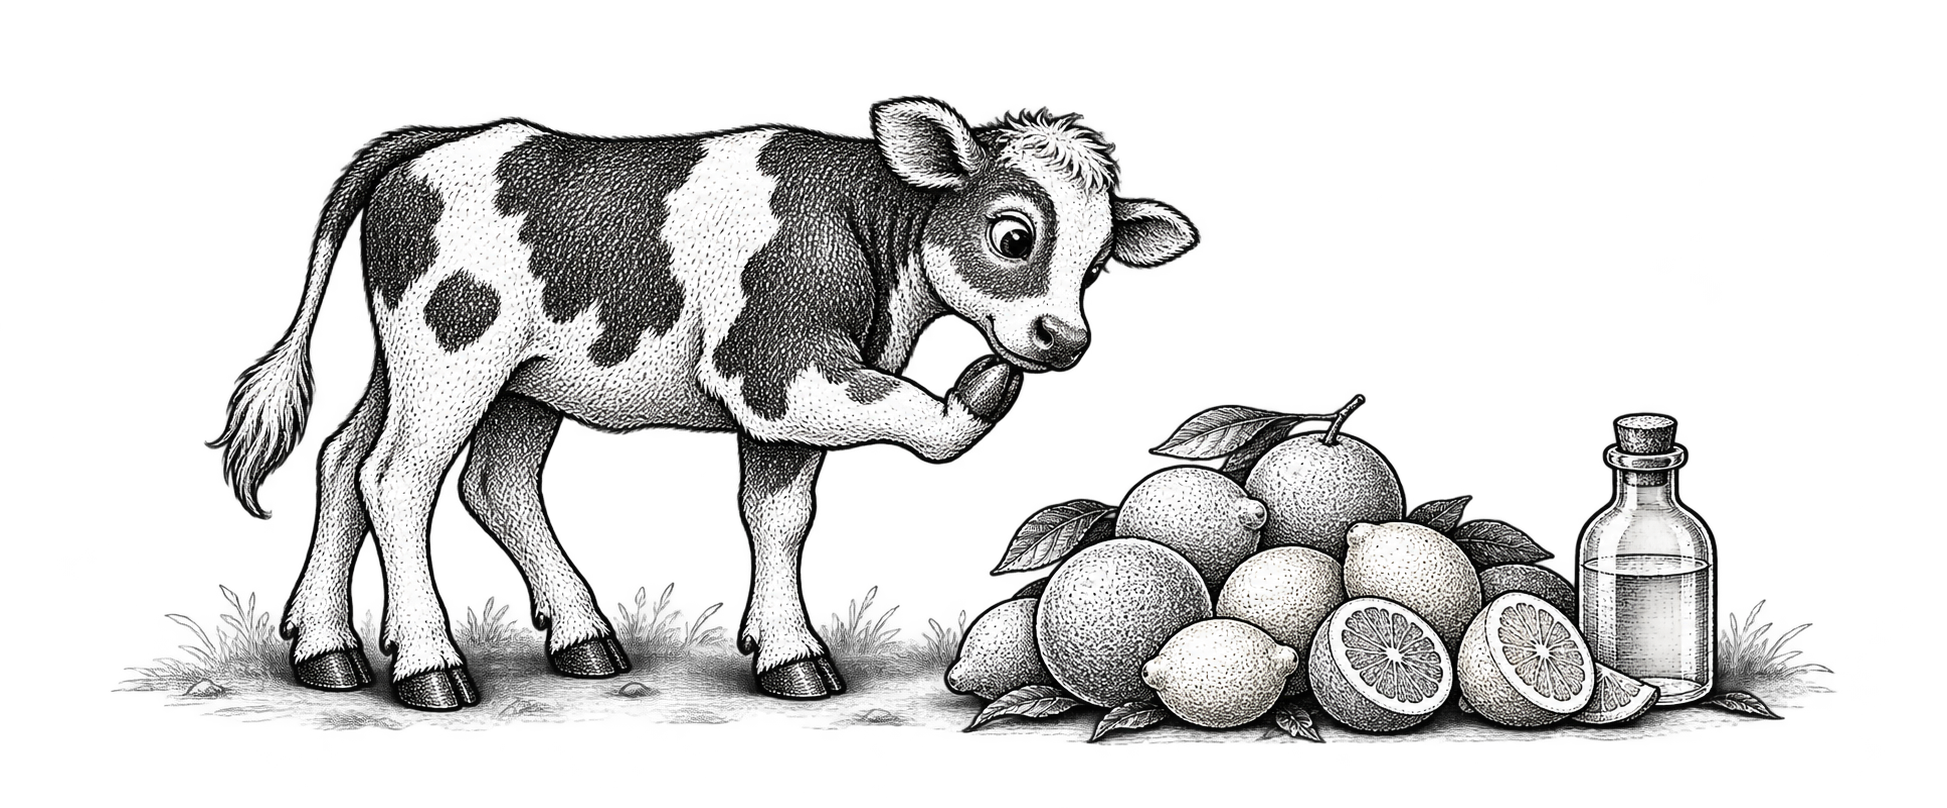
\includegraphics[width=174mm,height=94mm,keepaspectratio]{assets/cover.png}};
\node[anchor=north west,inner sep=0,text width=174mm] at ([xshift=18mm,yshift=-224mm]current page.north west)
{\fontsize{12}{16}\selectfont Understand what each step establishes\\and why it leads to the next.};
\node[anchor=west,inner sep=0] at ([xshift=18mm,yshift=-269mm]current page.north west)
{
\includegraphics[width=43mm]{assets/logo.png}};
\node[anchor=east,inner sep=0] at ([xshift=192mm,yshift=-269mm]current page.north west)
{
\includegraphics[width=62mm]{assets/julians-pathfinder-monochrome.pdf}};
\node[anchor=north west,inner sep=0,text width=174mm] at ([xshift=18mm,yshift=-244mm]current page.north west) {\fontsize{11}{14}\selectfont \href{https://colab.research.google.com/github/fifteen02/julians-pathfinder/blob/main/Lesson\%204/lesson.ipynb}{\underline{Open this lesson in Google Colab}}};
\end{tikzpicture}\clearpage
\markboth{Questions}{}\raggedbottom\setlength{\parskip}{4pt}
{\heavy\fontsize{16}{20}\selectfont Lesson 4 / Fruit Feast\par}\medskip
\par\noindent\begin{minipage}{\linewidth}
{\heavy\fontsize{12}{15}\selectfont Understand the fruit and water choices\par}\medskip
\textbf{L4-01 / Eating without going over}\par\smallskip Fullness starts at 0 and must never exceed 10. An orange adds 4 and a lemon adds 7. You may eat either fruit repeatedly. Without water, what fullness values are reachable?\par
\end{minipage}\par\vspace{4mm}
\par\noindent\begin{minipage}{\linewidth}
\textbf{L4-02 / Water can make room}\par\smallskip At most once, the cow may drink water. Water halves the current fullness, rounding down. With limit 10 and fruit sizes 4 and 7, find a route to fullness 10.\par
\end{minipage}\par\vspace{4mm}
\par\noindent\begin{minipage}{\linewidth}
\textbf{L4-03 / Same fullness, different choices}\par\smallskip A reachability flag is a yes/no answer: can the cow reach this situation? Compare fullness 4 with water still unused and fullness 4 after drinking. Do they allow the same next actions? Why would one flag called reachable[4] lose information we need?\par
\end{minipage}\par\vspace{4mm}
\par\noindent\begin{minipage}{\linewidth}
\textbf{L4-04 / A small recursive search}\par\smallskip Write feast\_cached(limit, a, b) using cached recursion. The helper asks: from fullness f, with used\_water saying whether the drink has been used, what is the greatest final fullness reachable? List every legal next action, including stopping. Explain why f and used\_water belong in the cache key.\par
\par\smallskip{\small\textbf{Start with:}}\par\smallskip\noindent\colorbox{codepaper}{\parbox{\dimexpr\linewidth-2\fboxsep\relax}{\small\ttfamily\raggedright def feast\_cached(limit, a, b):\\\hspace*{2.4em}def best(fullness, used\_water):\\\hspace*{4.8em}return None  \# Your helper goes here.\\\hspace*{2.4em}return best(0, False)}}\par
{\small\textbf{What each function returns.}\par feast\_cached(limit, a, b): the greatest reachable fullness, starting empty with water unused.\par best(fullness, used\_water): the greatest final fullness reachable from this fullness and water status.\par }
{\small\textbf{Hints.}}\begin{itemize}\item Stopping is always allowed. What does that give as a first answer?\item Which moves are legal from (fullness, used\_water)?\item Which move changes used\_water, and can it happen twice?\end{itemize}
\end{minipage}\par\vspace{4mm}
\par\noindent\begin{minipage}{\linewidth}
{\heavy\fontsize{12}{15}\selectfont Build the three passes\par}\medskip
\textbf{L4-05 / First, all fullness values before water}\par\smallskip For limit 10 and fruit sizes 4 and 7, fill dry[0] through dry[10]. Why can the scan run from low fullness to high fullness?\par
\par\medskip \begingroup\footnotesize\setlength{\tabcolsep}{4pt}\renewcommand{\arraystretch}{1.35}\begin{tabularx}{\linewidth}{>{\raggedright\arraybackslash}l>{\raggedright\arraybackslash}X>{\raggedright\arraybackslash}X>{\raggedright\arraybackslash}X>{\raggedright\arraybackslash}X>{\raggedright\arraybackslash}X>{\raggedright\arraybackslash}X>{\raggedright\arraybackslash}X>{\raggedright\arraybackslash}X>{\raggedright\arraybackslash}X>{\raggedright\arraybackslash}X>{\raggedright\arraybackslash}X}\toprule\textbf{Fullness f} & \textbf{0} & \textbf{1} & \textbf{2} & \textbf{3} & \textbf{4} & \textbf{5} & \textbf{6} & \textbf{7} & \textbf{8} & \textbf{9} & \textbf{10}\\\midrule
dry[f] & Y & ? & ? & ? & ? & ? & ? & ? & ? & ? & ?\\
\bottomrule\end{tabularx}\endgroup\par\medskip 
\end{minipage}\par\vspace{4mm}
\par\noindent\begin{minipage}{\linewidth}
\textbf{L4-06 / Then, drink from every dry state}\par\smallskip Take every fullness you marked as reachable without water in L4-05. Halve each one, rounding down, to find the states immediately after drinking and before any further fruit. Why would drinking only from the largest dry value miss a useful possibility?\par
\end{minipage}\par\vspace{4mm}
\par\noindent\begin{minipage}{\linewidth}
\textbf{L4-07 / Finally, eat after water}\par\smallskip Start from the values you found in L4-06 immediately after drinking. Fruit adds 4 or 7 and the limit is 10. Mark every fullness reachable after any further fruit, including no further fruit. A second drink is forbidden. What is the largest reachable fullness?\par
\par\medskip \begingroup\footnotesize\setlength{\tabcolsep}{4pt}\renewcommand{\arraystretch}{1.35}\begin{tabularx}{\linewidth}{>{\raggedright\arraybackslash}l>{\raggedright\arraybackslash}X>{\raggedright\arraybackslash}X>{\raggedright\arraybackslash}X>{\raggedright\arraybackslash}X>{\raggedright\arraybackslash}X>{\raggedright\arraybackslash}X>{\raggedright\arraybackslash}X>{\raggedright\arraybackslash}X>{\raggedright\arraybackslash}X>{\raggedright\arraybackslash}X>{\raggedright\arraybackslash}X}\toprule\textbf{Fullness f} & \textbf{0} & \textbf{1} & \textbf{2} & \textbf{3} & \textbf{4} & \textbf{5} & \textbf{6} & \textbf{7} & \textbf{8} & \textbf{9} & \textbf{10}\\\midrule
wet[f] &  &  &  &  &  &  &  &  &  &  & \\
\bottomrule\end{tabularx}\endgroup\par\medskip 
\end{minipage}\par\vspace{4mm}
\par\noindent\begin{minipage}{\linewidth}
\textbf{L4-08 / The complete three-pass program}\par\smallskip Write feast\_table(limit, a, b) with three passes: eat before water, drink once from each reachable value, then eat after water. A bytearray is a compact list of integers, initially all 0. Use 1 for reachable states. Explain the two arrays, scan order and choice of final answer.\par
\par\smallskip{\small\textbf{Start with:}}\par\smallskip\noindent\colorbox{codepaper}{\parbox{\dimexpr\linewidth-2\fboxsep\relax}{\small\ttfamily\raggedright def feast\_table(limit, a, b):\\\hspace*{2.4em}return None  \# Replace with your answer.}}\par
{\small\textbf{What each function returns.}\par feast\_table(limit, a, b): the greatest reachable fullness, starting empty with water unused.\par }
{\small\textbf{Hints.}}\begin{itemize}\item Which fullness is reachable before anything is eaten?\item Keep the three passes in order: eat, drink once, eat again.\item Which array does each pass read, and which does it write?\end{itemize}
\end{minipage}\par\vspace{4mm}
\par\noindent\begin{minipage}{\linewidth}
{\heavy\fontsize{12}{15}\selectfont Test and explain the pass order\par}\medskip
\textbf{L4-09 / Your turn: a different feast}\par\smallskip Use limit 9 and fruit sizes 4 and 6. Mark three rows: reachable without water; immediately after drinking; after any further fruit. Keep the water-only row separate from the completed wet row. Give a route to the largest final fullness. Test your feast\_table(limit, a, b) from L4-08 on this example.\par
\par\medskip \begingroup\footnotesize\setlength{\tabcolsep}{4pt}\renewcommand{\arraystretch}{1.35}\begin{tabularx}{\linewidth}{>{\raggedright\arraybackslash}l>{\raggedright\arraybackslash}X>{\raggedright\arraybackslash}X>{\raggedright\arraybackslash}X>{\raggedright\arraybackslash}X>{\raggedright\arraybackslash}X>{\raggedright\arraybackslash}X>{\raggedright\arraybackslash}X>{\raggedright\arraybackslash}X>{\raggedright\arraybackslash}X>{\raggedright\arraybackslash}X}\toprule\textbf{Fullness f} & \textbf{0} & \textbf{1} & \textbf{2} & \textbf{3} & \textbf{4} & \textbf{5} & \textbf{6} & \textbf{7} & \textbf{8} & \textbf{9}\\\midrule
dry[f] & Y &  &  &  &  &  &  &  &  & \\
just drank &  &  &  &  &  &  &  &  &  & \\
wet[f] &  &  &  &  &  &  &  &  &  & \\
\bottomrule\end{tabularx}\endgroup\par\medskip 
\end{minipage}\par\vspace{4mm}
\par\noindent\begin{minipage}{\linewidth}
\textbf{L4-10 / Boundary tests and optional water}\par\smallskip Test your feast\_table(limit, a, b) from L4-08. Here limit is maximum fullness, and a and b are the fruit increases. First predict the answers for (1, 1, 1), (8, 4, 6) and (5, 4, 4), then run your function. Must the cow drink? Give a route for each answer.\par
\end{minipage}\par\vspace{4mm}
\par\noindent\begin{minipage}{\linewidth}
\textbf{L4-11 / Explain why the pass order works}\par\smallskip Why must all states reachable without water be found before we halve them, and all immediate-after-water states be marked before we add more fruit? Use the path 0 to 7, drink to 3, then add 7 as an example of the required order.\par
\end{minipage}\par\vspace{4mm}
\end{document}